\appendix 
\chapter{Documentación de la aplicación distribuida}
\section{Javadoc}
Javadoc es una utilidad de Oracle para la generación de documentación de APIs en formato HTML a partir de código fuente Java. Javadoc es el estándar de la industria para documentar clases de Java. La mayoría de los IDEs los generan automáticamente.\\ \\
A continuación se explican algunas de las palabras reservadas:
\begin{table}[h!]
	\centering
	\rowcolors{1}{white}{claro}
	\setlength\arrayrulewidth{1.2pt}
	\begin{tabular}{p{4cm} @{\hspace{1mm}}p{9cm}}
		\hline Tag & Descripción\\
		\hline @author & Nombre del desarrollador\\
		@deprecated & Indica que el método o clase es antigua y que no se recomienda su uso porque posiblemente desaparecerá en versiones posteriores\\
		@param & Definición de un parámetro de un método, es requerido para todos los parámetros del método\\
		@return & Informa de lo que devuelve el método, no se puede usar en constructores o métodos "void"\\
		@see & Asocia con otro método o clase\\
		@throws & Excepción lanzada por el método\\
		@version & Versión del método o clase\\
		\hline
	\end{tabular}
	\caption{Uso de los tags}
	\label{tabla:formato_javadoc}
\end{table}

\section{Documentación}
\label{javadoc}
En las siguientes páginas se puede ver la documentación de la aplicación.
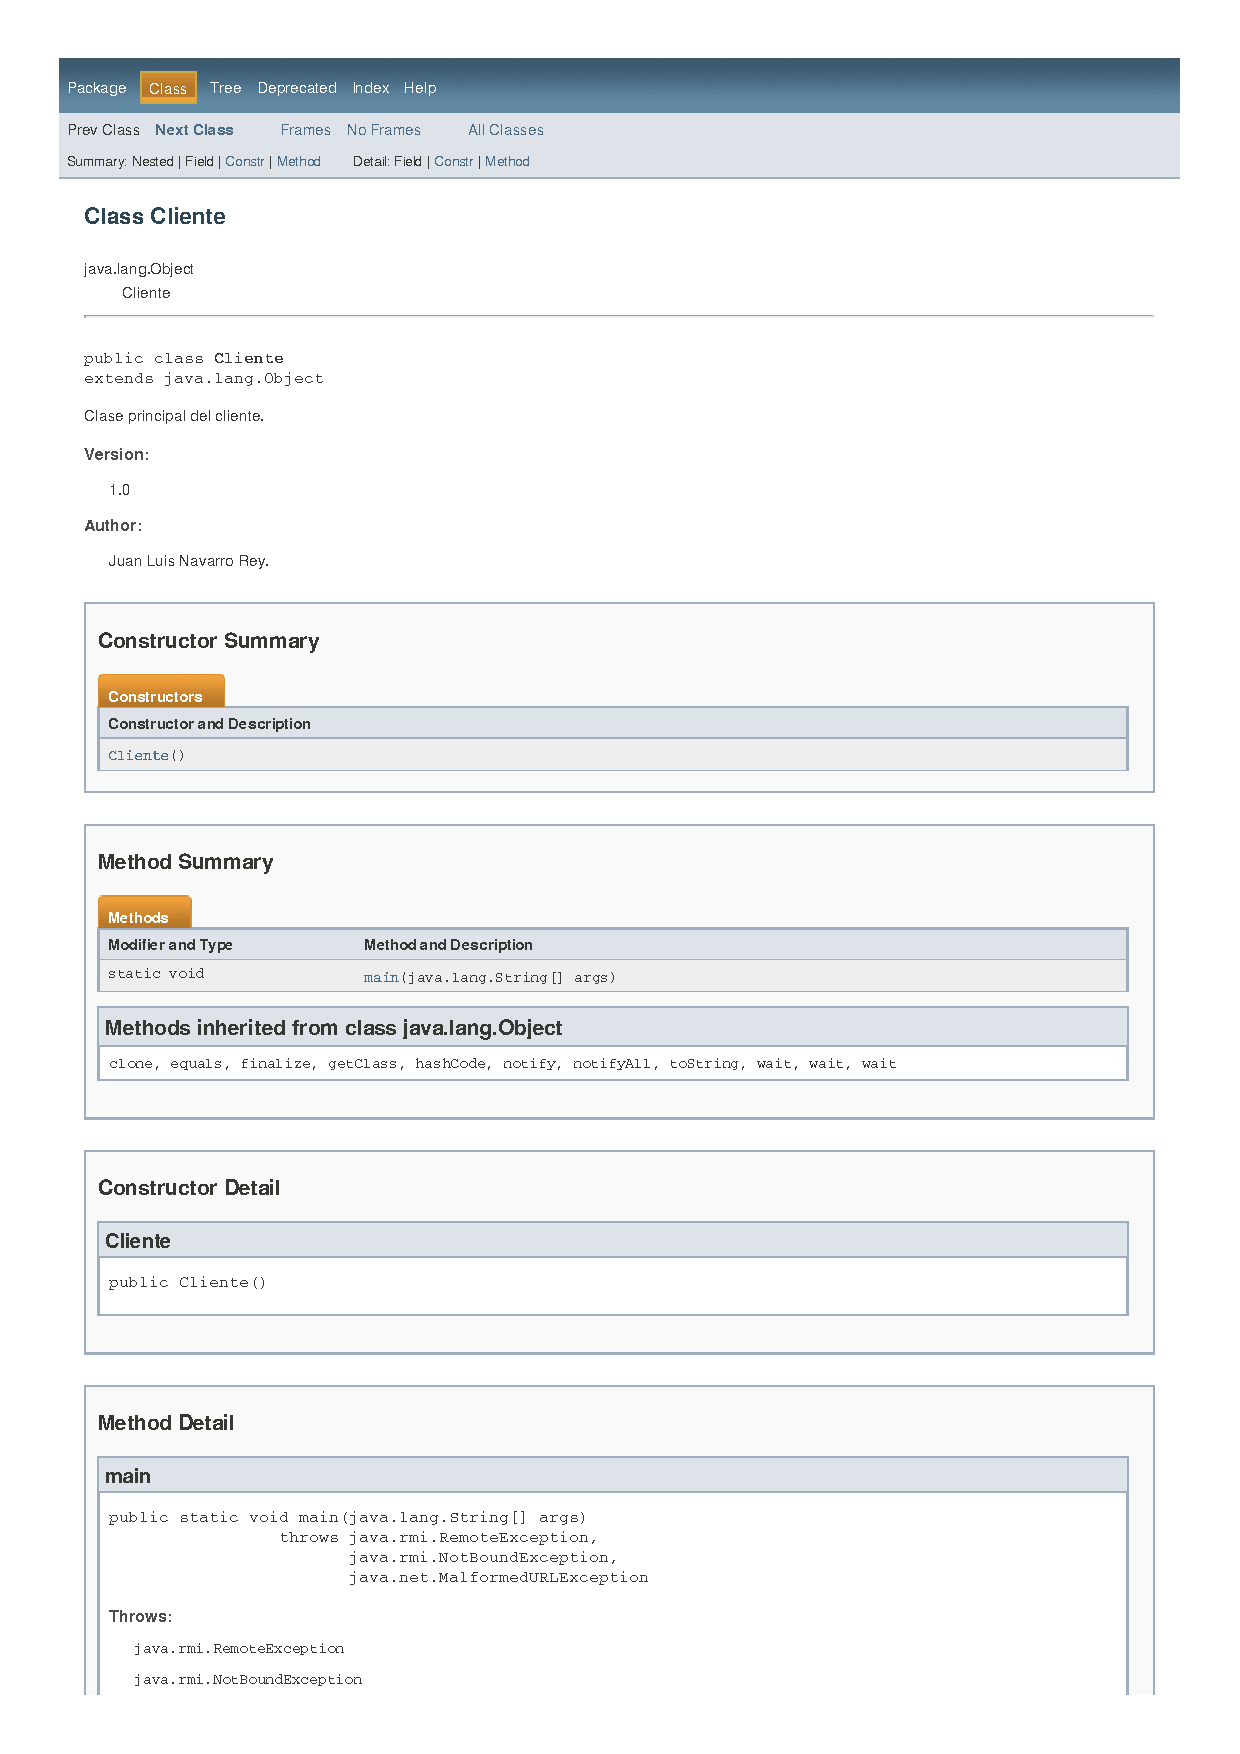
\includepdf[pages=-,nup=1x1,frame=false,scale=0.9,pagecommand={\label{doc:cliente}}]{javadoc/Cliente.pdf}
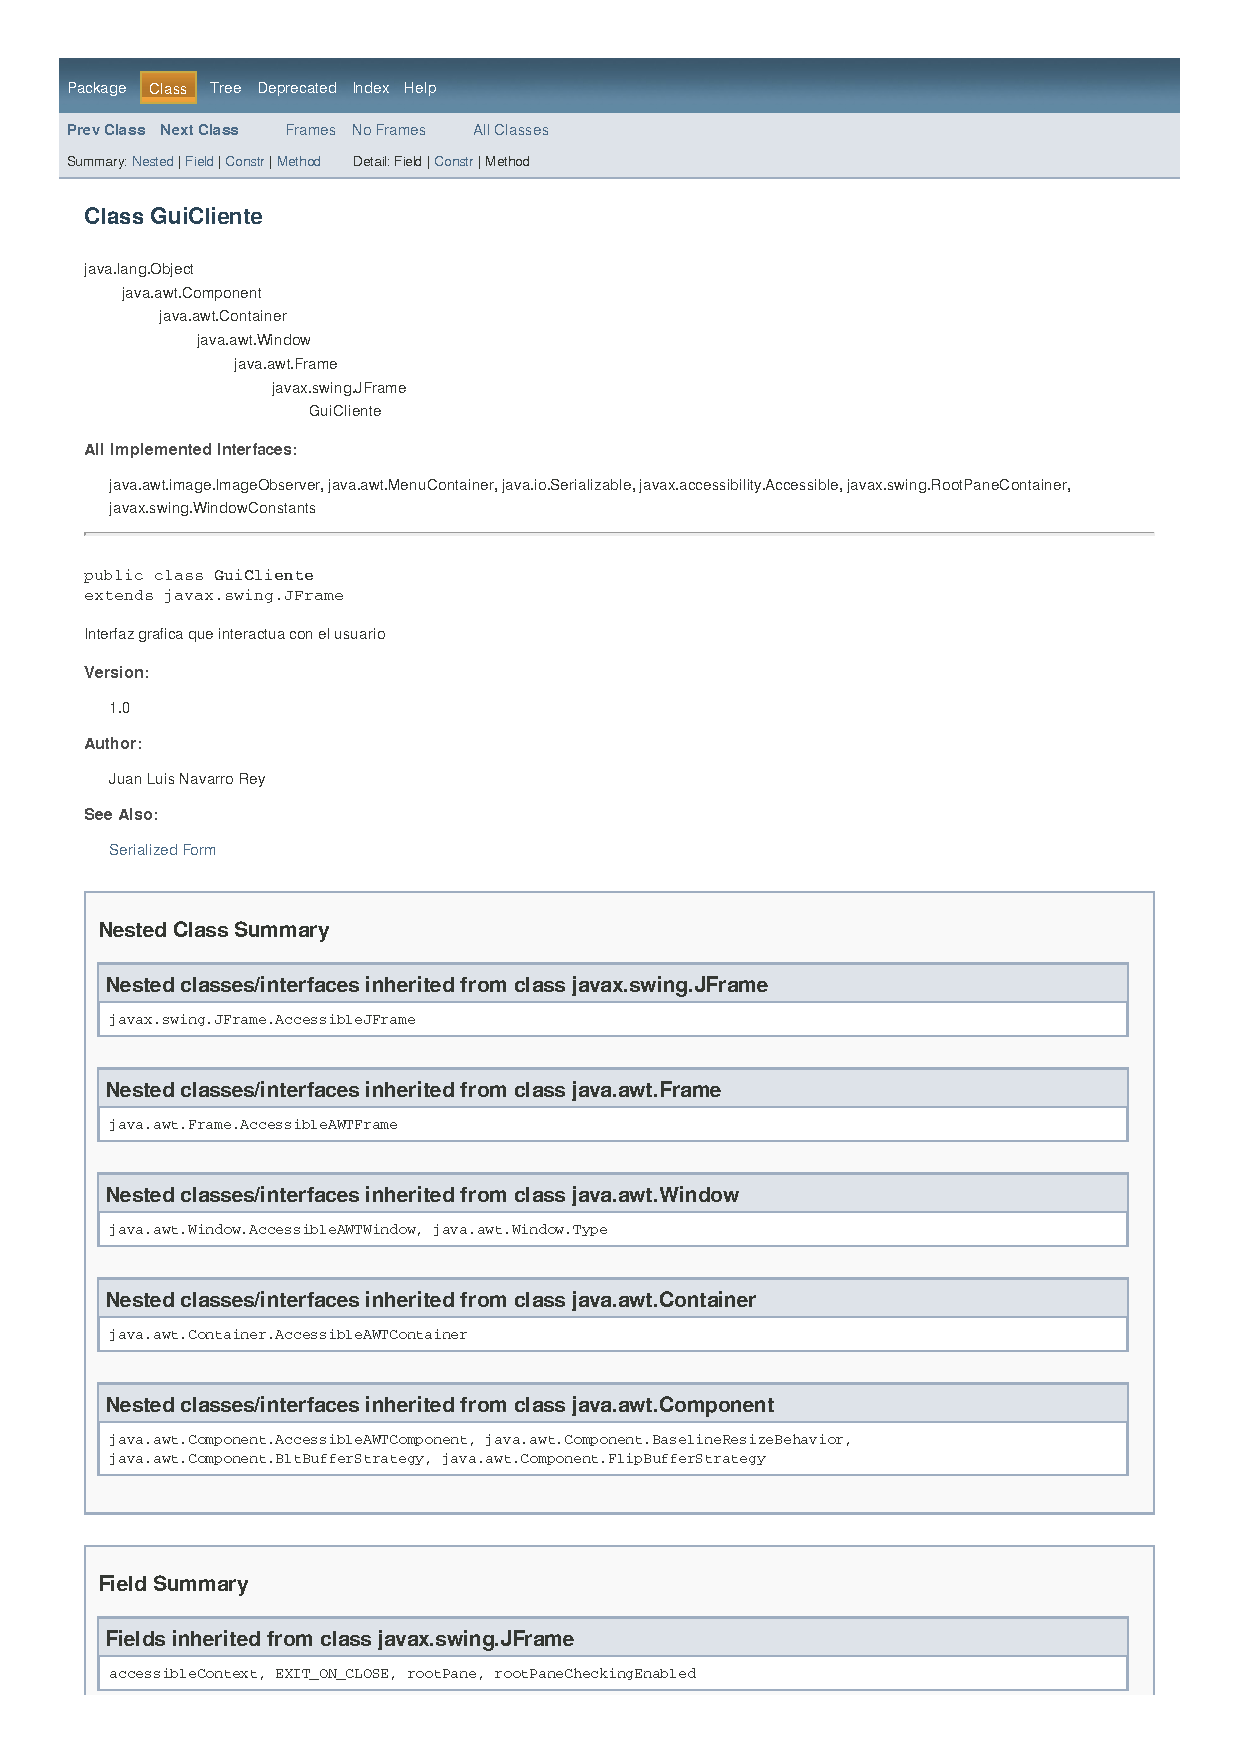
\includepdf[pages=-,nup=1x1,frame=false,scale=0.9,pagecommand={\label{doc:guicliente}}]{javadoc/GuiCliente.pdf}
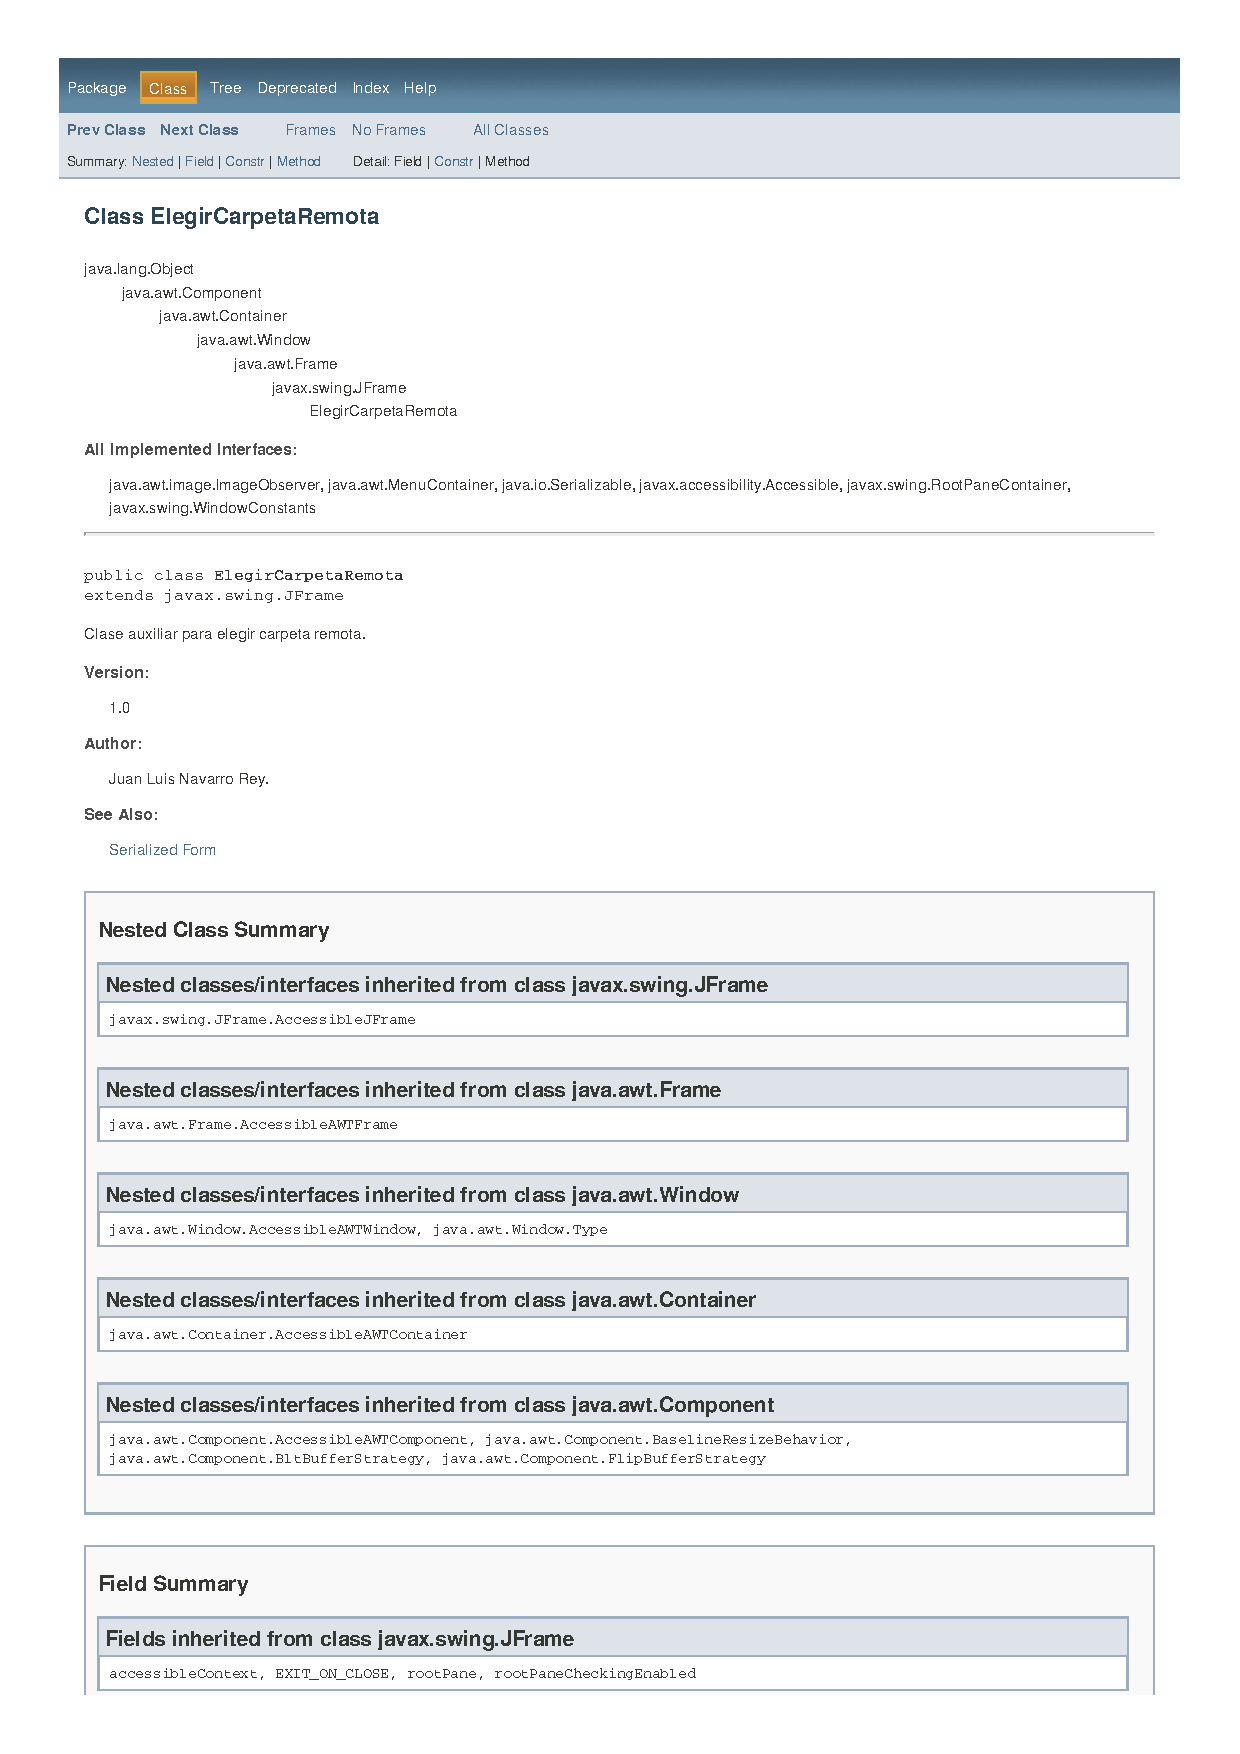
\includepdf[pages=-,nup=1x1,frame=false,scale=0.9,pagecommand={\label{doc:elegircarpetaremota}}]{javadoc/ElegirCarpetaRemota.pdf}
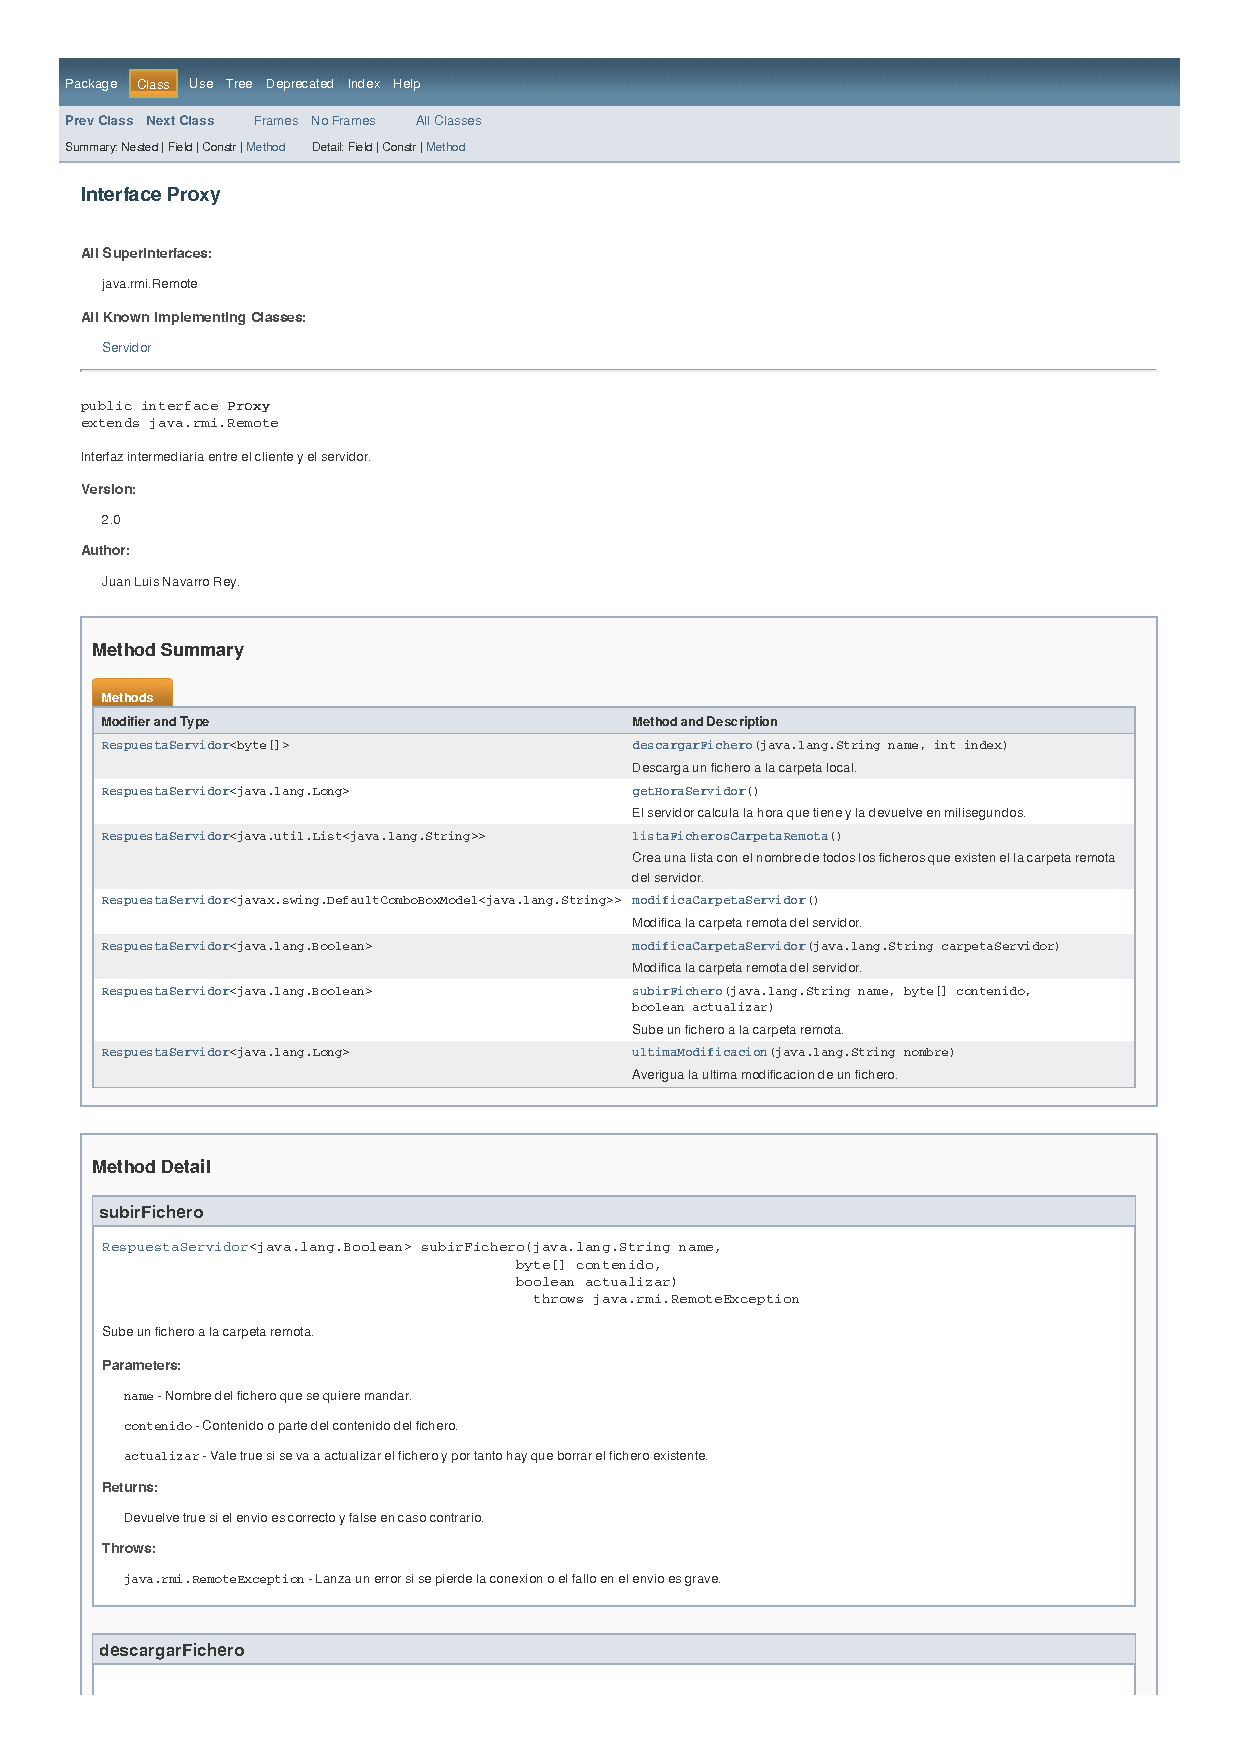
\includepdf[pages=-,nup=1x1,frame=false,scale=0.9,pagecommand={\label{doc:proxy}}]{javadoc/Proxy.pdf}
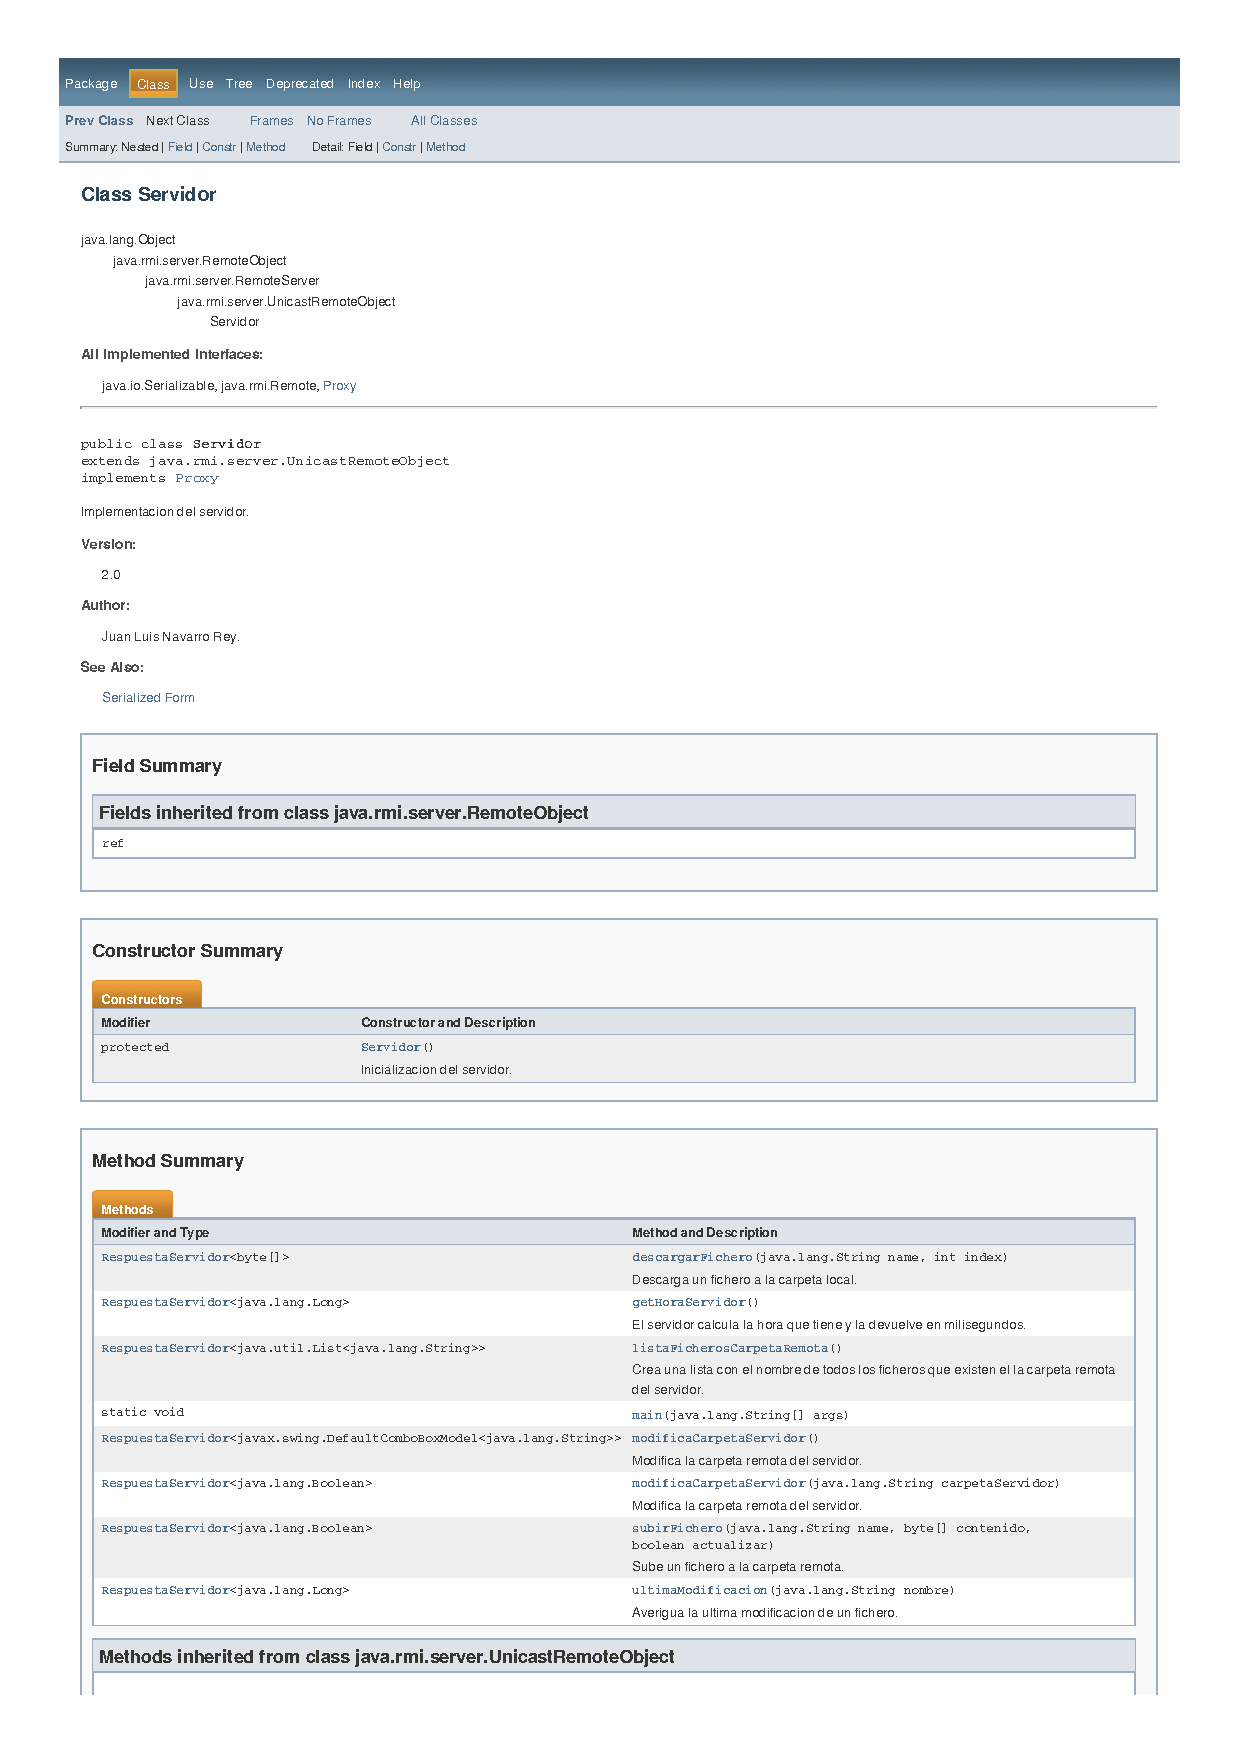
\includepdf[pages=-,nup=1x1,frame=false,scale=0.9,pagecommand={\label{doc:servidor}}]{javadoc/Servidor.pdf}
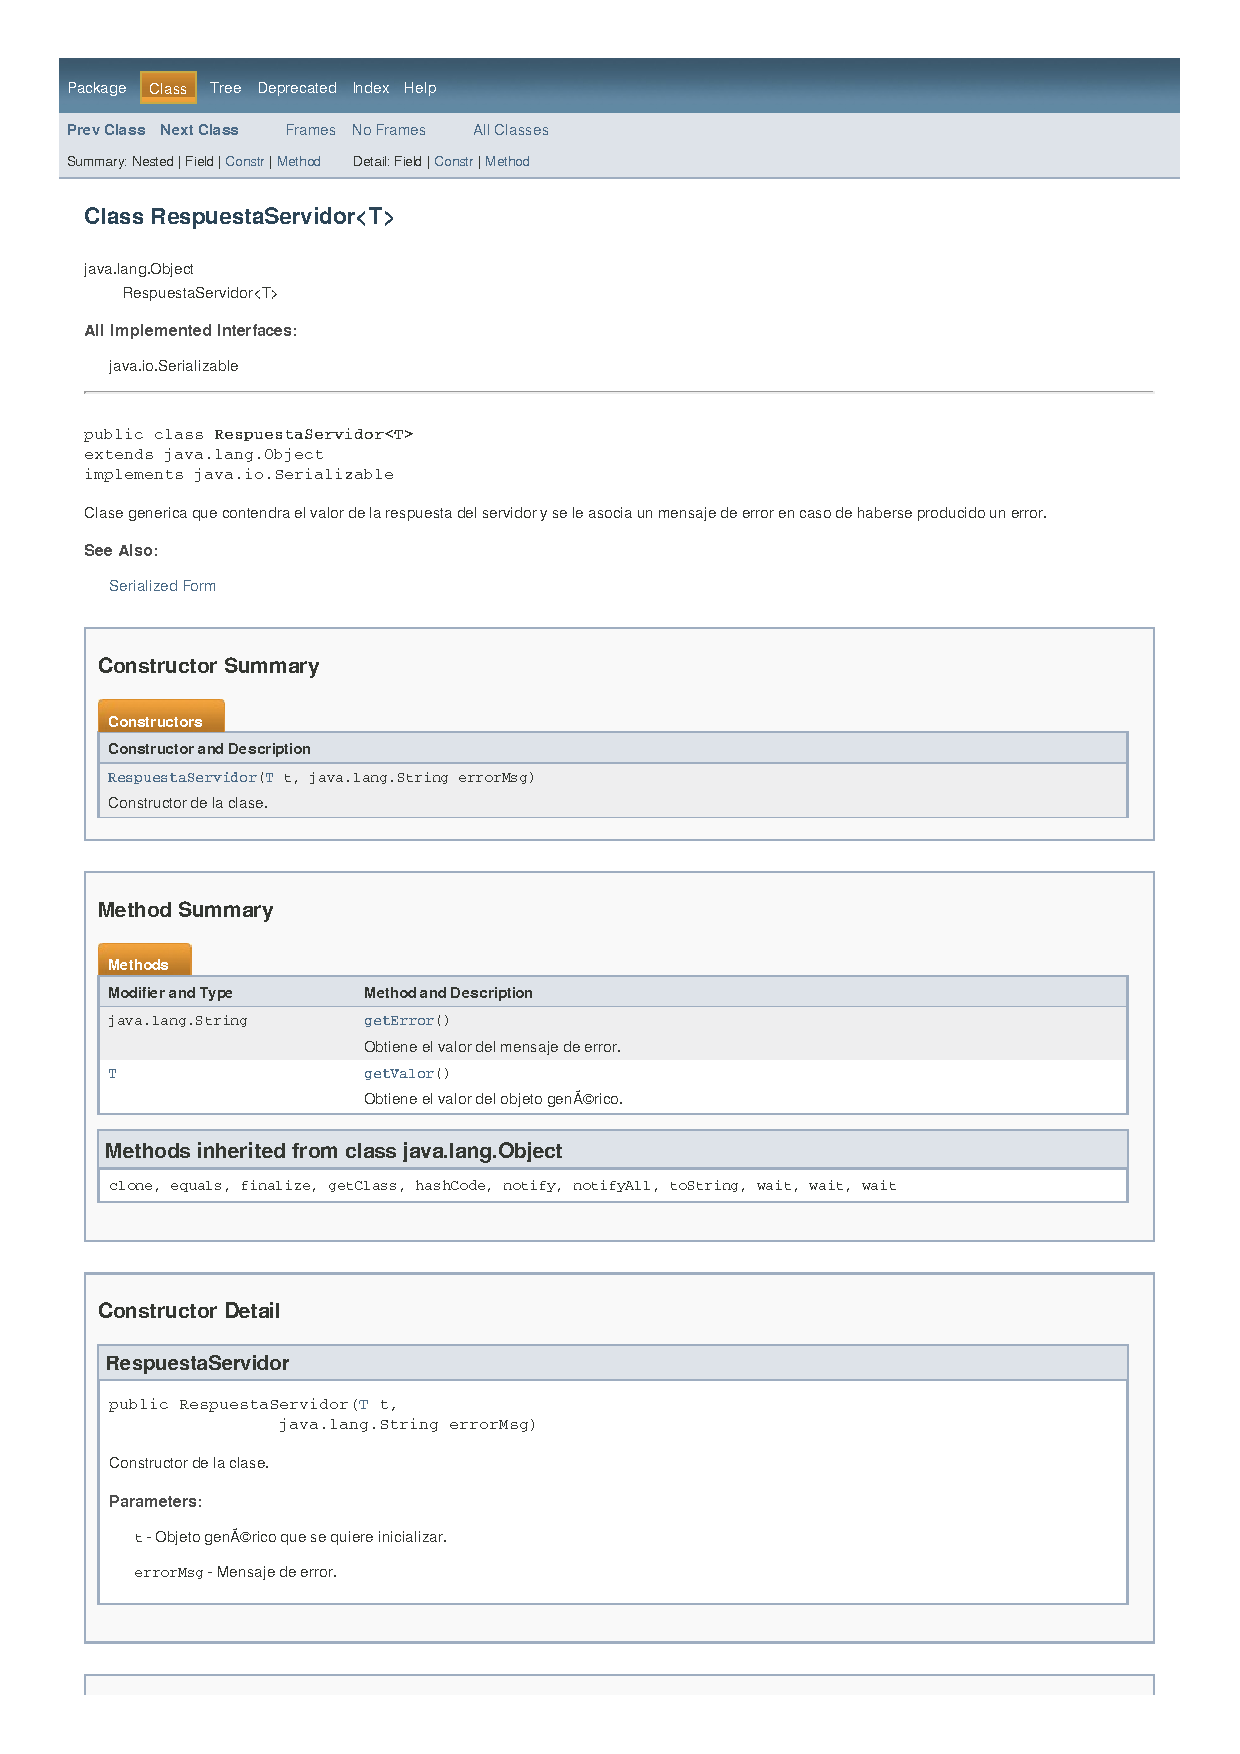
\includepdf[pages=-,nup=1x1,frame=false,scale=0.9,pagecommand={\label{doc:respuestaservidor}}]{javadoc/RespuestaServidor.pdf}
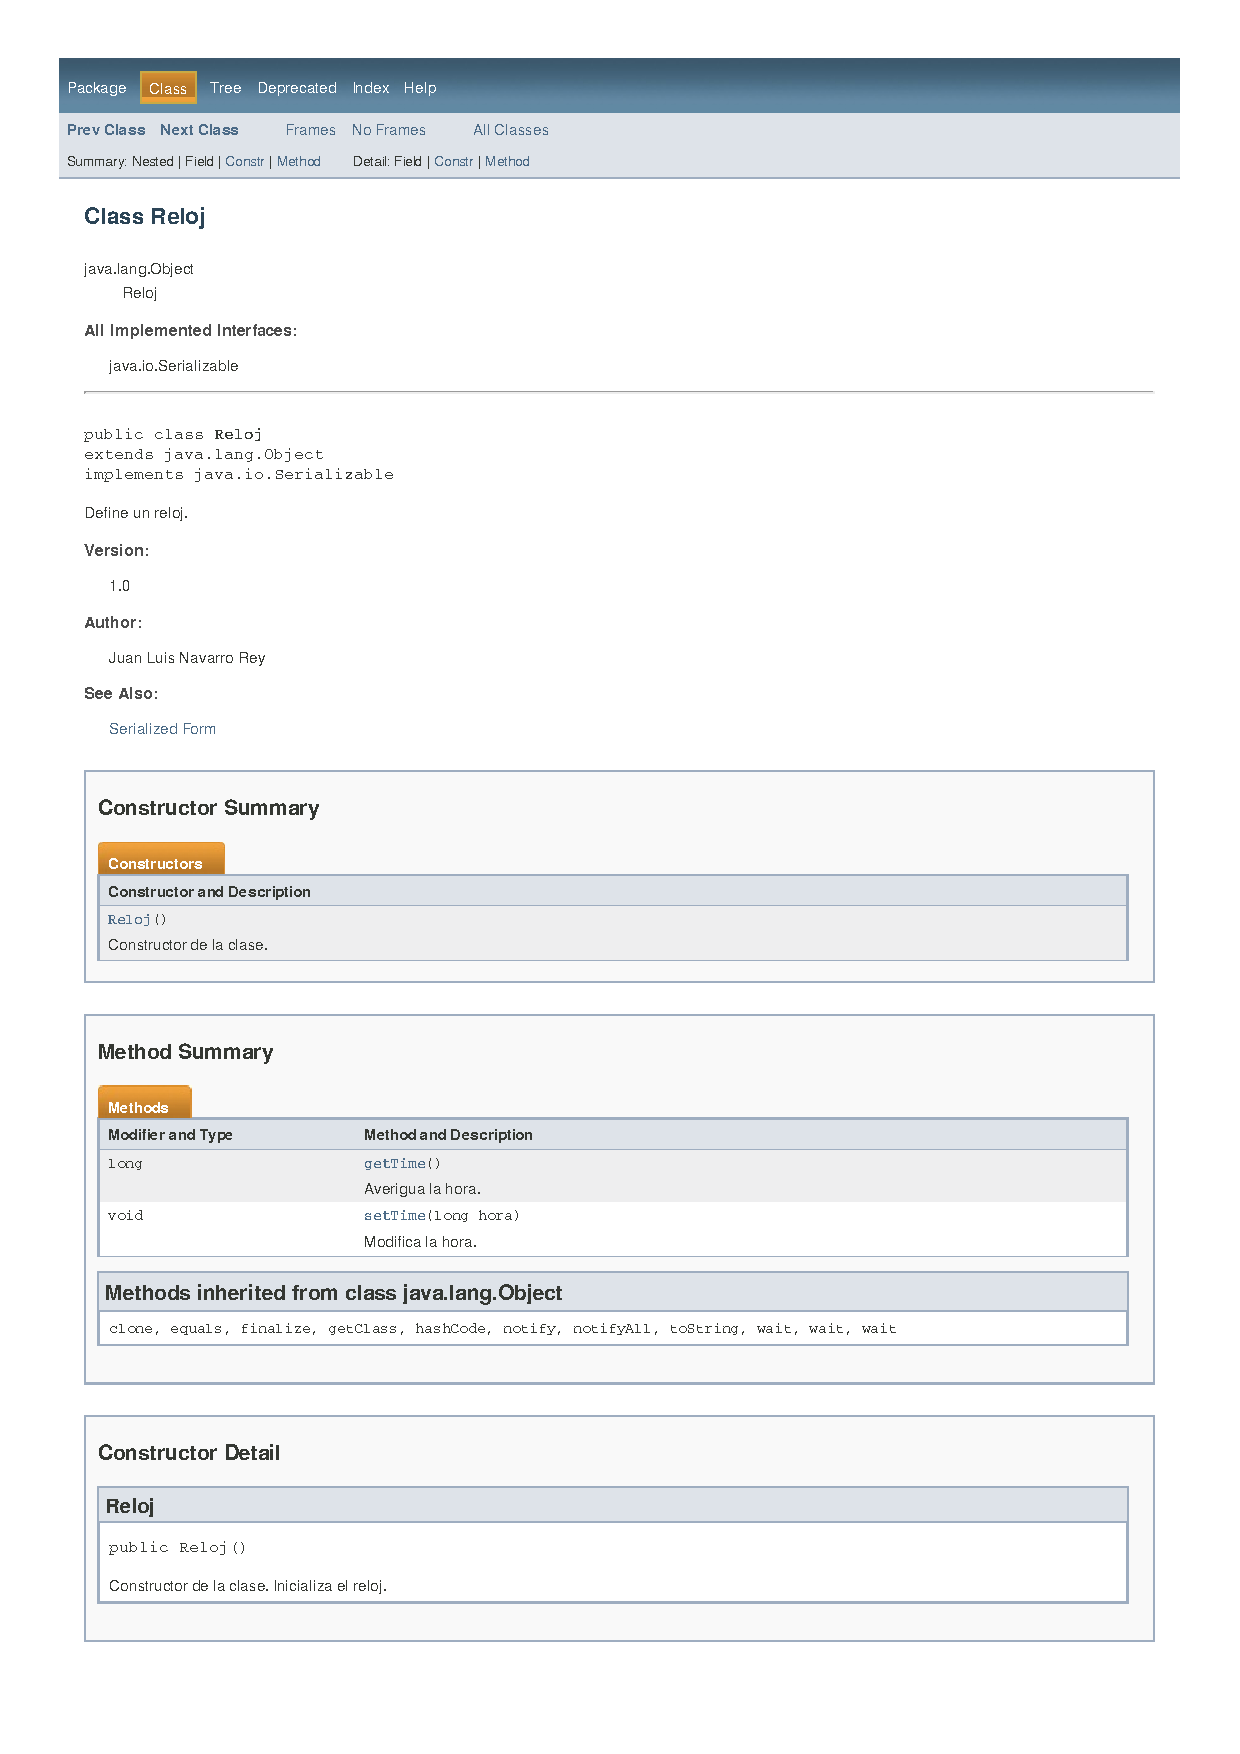
\includepdf[pages=-,nup=1x1,frame=false,scale=0.9,pagecommand={\label{doc:reloj}}]{javadoc/Reloj.pdf}